\documentclass[unknownkeysallowed]{beamer}

\usetheme{qrmMMXV}
\usecolortheme{qrmMMXV}

% arrays

\newcommand{\otoprule}{\midrule[\heavyrulewidth]}

% font

\ifxetex
% if you use xelatex for compiling, then you can set a FreeType font
% like this
\usepackage{fontspec}
% \setmainfont[Mapping=tex-text]{Gill Sans MT Std}
 \setmainfont[Mapping=tex-text]{Bryant Pro}
% \setmainfont[Mapping=tex-text]{Ubuntu}
\let\sfdefault\rmdefault
\fi

% color settings

\usepackage{color,colortbl}
\usepackage{xspace}
\definecolor{gray98}{rgb}{0.98,0.98,0.98}
\definecolor{gray20}{rgb}{0.20,0.20,0.20}
\definecolor{gray25}{rgb}{0.25,0.25,0.25}
\definecolor{gray16}{rgb}{0.161,0.161,0.161}
\definecolor{gray60}{rgb}{0.6,0.6,0.6}
\definecolor{gray30}{rgb}{0.3,0.3,0.3}
\definecolor{bgray}{RGB}{248, 248, 248}
\definecolor{amgreen}{RGB}{77, 175, 74}
% \definecolor{amblu}{RGB}{72, 88, 102}
\definecolor{amblu}{RGB}{55, 126, 184}
\definecolor{amred}{RGB}{228,26,28}
\definecolor{amyellow}{RGB}{237,177,32}
\definecolor{ampurple}{RGB}{126,47,142}

\newcommand{\dg}[1]{\textcolor{mgreen}{#1\xspace}}
\newcommand{\dr}[1]{\textcolor{mred}{#1\xspace}}
\newcommand{\db}[1]{\textcolor{mblue}{#1\xspace}}
\newcommand{\dd}[1]{\textcolor{gray!70}{#1\xspace}}
\newcommand{\gn}[1]{\textcolor{gray!110}{#1\xspace}}
\newcommand{\gs}[1]{\textcolor{gray!50}{#1\xspace}}
\newcommand{\gt}[1]{\textcolor{gray!20}{#1\xspace}}
\newcommand{\dk}[1]{\textcolor{black}{#1\xspace}}

\newcommand{\mye}[1]{\textcolor{amyellow}{#1}\xspace}
\newcommand{\mgr}[1]{\textcolor{amgreen}{#1}\xspace}
\newcommand{\mbl}[1]{\textcolor{amblu}{#1}\xspace}
\newcommand{\mre}[1]{\textcolor{amred}{#1}\xspace}
\newcommand{\mbk}[1]{\textcolor{black}{#1}\xspace}
\newcommand{\mbp}[1]{\textcolor{ampurple}{#1}\xspace}

% citations

\newcommand{\mycite}[1]{[{\scriptsize #1}]}

% source code

\usepackage[procnames]{listings}
\lstset{ %
  backgroundcolor=\color{gray98},    % choose the background color; you must add \usepackage{color} or \usepackage{xcolor}
  basicstyle=\tt\tiny, % \prettysmall      % the size of the fonts that are used for the code
  breakatwhitespace=false,          % sets if automatic breaks should only happen at whitespace
  breaklines=true,                  % sets automatic line breaking
  showlines=false,                  % sets automatic line breaking
  captionpos=b,                     % sets the caption-position to bottom
  commentstyle=\color{gray30},      % comment style
  extendedchars=true,               % lets you use non-ASCII characters; for 8-bits encodings only, does not work with UTF-8
  frame=single,                     % adds a frame around the code
  keepspaces=true,                  % keeps spaces in text, useful for keeping indentation of code (possibly needs columns=flexible)
  keywordstyle=\color{amblu},       % keyword style
  procnamestyle=\color{amred},      % procedures style
  language=[95]fortran,             % the language of the code
  numbers=none,                     % where to put the line-numbers; possible values are (none, left, right)
  numbersep=5pt,                    % how far the line-numbers are from the code
  numberstyle=\tiny\color{gray20},  % the style that is used for the line-numbers
  rulecolor=\color{gray20},         % if not set, the frame-color may be changed on line-breaks within not-black text (e.g. comments (green here))
  showspaces=false,                 % show spaces everywhere adding particular underscores; it overrides 'showstringspaces'
  showstringspaces=false,           % underline spaces within strings only
  showtabs=false,                   % show tabs within strings adding particular underscores
  stepnumber=2,                     % the step between two line-numbers. If it's 1, each line will be numbered
  stringstyle=\color{amblu},        % string literal style
  tabsize=2,                        % sets default tabsize to 2 spaces
  title=\xspace,                    % show the filename of files included with \lstinputlisting; also try caption instead of title
  procnamekeys={call},
  keywords=[2]{R, W, RW},
}

% additional commands

\newcommand{\qrm}{\texttt{qr\_mumps}\xspace}
\newcommand{\qrs}{\texttt{qr\_starpu}\xspace}
\newcommand{\spqr}{\texttt{SPQR}\xspace}
\newcommand{\spqrgpu}{\texttt{SPQRGPU}\xspace}
\newcommand\ignore[1]{{}}
\newcommand{\starpu}{{StarPU}\xspace}

%% For additional slides 

\newcommand{\AdditionalSlidesBegin}{
   \newcounter{framenumbervorappendix}
   \setcounter{framenumbervorappendix}{\value{framenumber}}
}
\newcommand{\AdditionalSlidesEnd}{
   \addtocounter{framenumbervorappendix}{-\value{framenumber}}
   \addtocounter{framenumber}{\value{framenumbervorappendix}} 
}

\author{Iain S. Duff, Jonathan D. Hogg and {\bf Florent Lopez}} 

\institute{Rutherford Appleton Laboratory
  \\ \alert{NLAFET Project}}

\title{Task-based Sparse Cholesky Solver on Top of Runtime System}

\date{PMAA'16, 2016}

\begin{document}

\begin{frame}[t,plain]
\titlepage
\end{frame}

\begin{frame}{Objective}

  Solve \alert{$Ax=b$}, where $A$ is \db{large} and \db{sparse}, on
  modern architectures.

  \vspace{0.5cm}
  
  Using \db{Direct Method}: Sparse Cholesky factorization $A=LL^{T}$
  \begin{itemize}
  \item[\dg{$\blacktriangle$}] Numerically robust and general purpose
  \item[\dr{$\blacktriangledown$}] High memory usage and computational cost
  \end{itemize}

  \vspace{0.5cm}

  Exploiting modern platforms is challenging:
  \begin{itemize}
  \item \db{Multicore} processors and deep \db{memory hierarchy}.
  \item \db{Heterogeneous} e.g. CPU \& GPU or Xeon Phi.
  \item \db{Distributed-memory} systems. 
  \end{itemize}

\end{frame}

\begin{frame}{Runtime systems}
  \begin{columns}
    \begin{column}{0.45\textwidth}
      \center
      \only<1>{\includegraphics[width=\textwidth]{figures/rt_layers1}}%
      \only<2->{\includegraphics[width=\textwidth]{figures/rt_layers2}}%
    \end{column}
    \begin{column}{0.55\textwidth}
      \begin{itemize}
      \item<1->The classical approach is based on a mixture of
        technologies (e.g., MPI+OpenMP+CUDA) which.
        \begin{itemize}
        \item programming costs.
        \item is difficult to maintain and update.
        \item is prone to (performance) portability issues.
        \end{itemize}
      \item<2-> runtimes provide an abstraction layer that hides the
        architecture details.
      \item<3-> the workload is expressed as a DAG of tasks.
        % where the dependencies are
        % \begin{itemize}
        % \item<3-> defined explicitly
        % \item<3-> defined through rules
        % \item<3-> automatically inferred
        % \end{itemize}
      \end{itemize}
    \end{column}
  \end{columns}
\end{frame}

\begin{frame}{Sparse Cholesky factorization}
  
  \begin{columns}  

    \begin{column}{0.6\textwidth}  

      In numerical factorization of \alert{$A$} the
      \db{\textit{elimination tree}} expresses data dependencies in
      the factor \alert{$L$}. Each node, referred to as
      \db{\textit{supernode}}, is a \alert{dense} lower trapezoidal
      \alert{submatrix} of \alert{$L$}.

      \vspace{0.4cm}

      The tree is traversed in a \db{topological order}, and each node is
      factorized using \alert{dense Cholesky algorithm}.

      \vspace{0.4cm}
      
      Updates between node are handled using a \alert{supernodal scheme}
      i.e. updates are applied directly to the target supernodes.
    \end{column}

    \begin{column}{0.4\textwidth}  
      \only<1>{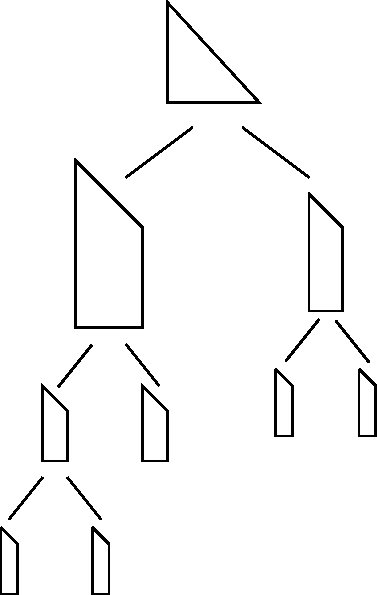
\includegraphics[width=0.9\textwidth]{figures/etree}}%
      \only<2>{\includegraphics[width=0.9\textwidth]{figures/etree2}}%
      \only<3>{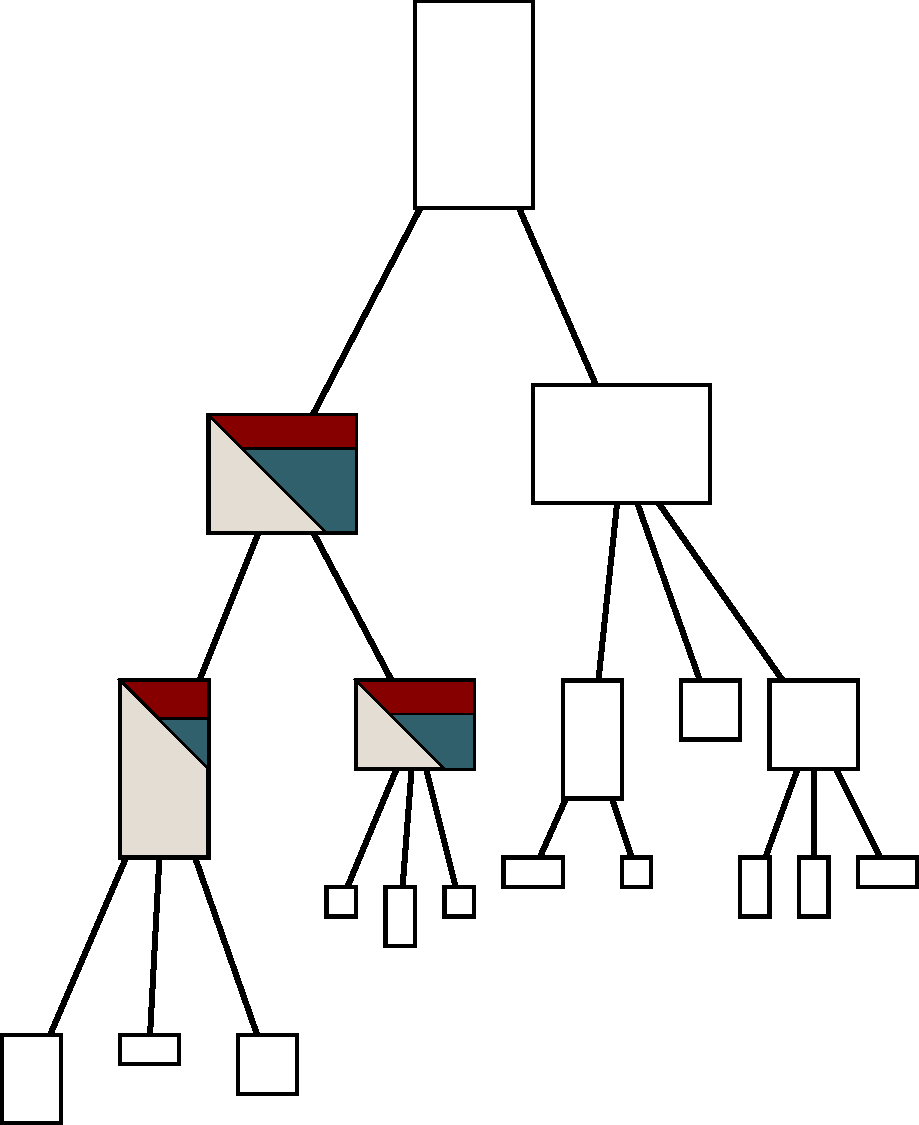
\includegraphics[width=0.9\textwidth]{figures/etree3}}%
    \end{column}

    \end{columns}

\end{frame}

\begin{frame}{Sparse Cholesky factorization: parallelism}
  
  \begin{columns}  

    \begin{column}{0.6\textwidth}  

      Sources of \alert{parallelism} in the elimination tree:
      \begin{itemize}
        \item<2-> \db{Tree parallelism}: Supernode in independent branches
          can be processed \alert{concurrently}.
        \item<3-> \db{Node parallelism}: When a supernode is large enough,
          it may be processed in parallel.
      \end{itemize}
    \end{column}

    \begin{column}{0.4\textwidth}  
      \only<1>{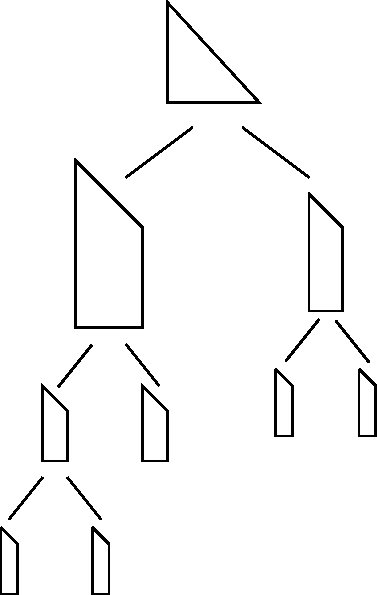
\includegraphics[width=0.9\textwidth]{figures/etree}}%
      \only<2>{\includegraphics[width=0.9\textwidth]{figures/etree_tree_para}}%
      \only<3>{\includegraphics[width=0.9\textwidth]{figures/etree_node_para}}%
    \end{column}

  \end{columns}

\end{frame}

\begin{frame}{Task-based Sparse Cholesky factorization}

  \begin{columns}
    \begin{column}{0.5\textwidth}
      \centering
      \only<1>{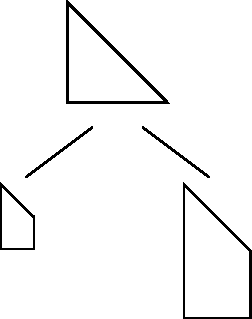
\includegraphics[width=0.6\textwidth]{figures/etree_simple}}%
      \only<2->{\includegraphics[width=0.6\textwidth]{figures/etree_simple_part}}%
    \end{column}

    \begin{column}{0.5\textwidth}
      \uncover<3->{\includegraphics[width=0.8\textwidth]{figures/dag}}%
    \end{column}

  \end{columns}
  
  \vspace{0.2cm}
  
  \uncover<2->{Supernodes are \alert{partitioned} into square
    \db{blocks} (\texttt{nb x nb}) on which operations are applied
    (\texttt{factorize}, \texttt{solve}, \texttt{update},
    \texttt{update\_between}).}\uncover<3->{ The \alert{DAG} replaces the
    elimination tree for representing the dependencies.}

  \uncover<4->{Implemented in the HSL package \db{MA87}.}

\end{frame}

%% \begin{frame}{Task-based Sparse Cholesky factorization}
%%   \only<1>{\lstinputlisting{listings/spllt-seq.F90}}
%%   \only<2>{\lstinputlisting{listings/spllt-task-seq.F90}}
%% \end{frame}

\begin{frame}{Task-based Sparse Cholesky factorization}
  \begin{columns}
    \begin{column}{0.6\textwidth}
      \only<1>{
        \lstinputlisting{listings/spllt-seq.F90}}
      \only<2>{\lstinputlisting{listings/spllt-task-seq.F90}}
    \end{column}
    \begin{column}{0.4\textwidth}
      \centering
      \only<1>{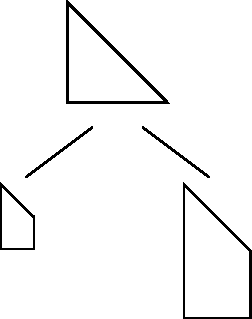
\includegraphics[width=0.6\textwidth]{figures/etree_simple}}%
      \only<2->{\includegraphics[width=0.6\textwidth]{figures/etree_simple_part}}%
    \end{column}
  \end{columns}
\end{frame}

\begin{frame}{The Sequential Task Flow Model}  
  \alert{Sequential Task Flow} (STF) programming model:

  \begin{itemize}
  \item In the parallel code, tasks are submitted to the runtime
    system following the \db{sequential algorithm}.
    \vspace{0.2cm}
  \item The runtime analyses the manipulated data and infers task
    dependencies in order to ensure the \db{sequential consistency} of
    the parallel code.
    \vspace{0.2cm}
  \item \db{Superscalar analysis} in processors: dependency detection
    between instructions in order to issue them in parallel.
    \vspace{0.2cm}
  \item The DAG is executed via a \db{dynamic scheduling} of the
    (ready) tasks on the architecture.
    \vspace{0.2cm}
  \item The runtime may be capable of automatically handling the
    \db{data transfers} on the architecture (e.g. CPU/GPU memory
    nodes).
    \vspace{0.2cm}
  \end{itemize} 
\end{frame}

\begin{frame}[fragile,t]{STF Sparse Cholesky Factorization}
      \only<1>{\lstinputlisting{listings/spllt-task-seq2.F90}}
      \only<2>{\lstinputlisting{listings/spllt-stf.F90}}
\end{frame}

\begin{frame}{STF on top of Runtime System}
  \alert{OpenMP 4.0}
  \begin{itemize}
  \item \texttt{task} construct and \texttt{depend} clause (\texttt{in}, \texttt{out},
    \texttt{inout}).
  \item No control on the scheduling policy.
  \item Shared-memory system only.
  \end{itemize}

  \vspace{0.5cm}

  \alert{StarPU}
  \begin{itemize}
  \item \texttt{starpu\_insert\_task} and data \textit{handle} with
    access mode (\texttt{R}, \texttt{W}, \texttt{RW}).
  \item Full control on schduling policy with possibility to implement
    new one.
  \item API for distributed-memory systems.
  \end{itemize}  
\end{frame}

\begin{frame}{Experiments}
  \texttt{\scriptsize
    \begin{tabular}{rlrl}
        \hline
        \# & Matrix                         & Flops ($10^{9}$) & Application/description  \\
        \hline
        1  & Schmid/thermal2                & 18.6             & Unstructured thermal FEM \\
        2  & Rothberg/gearbox               & 22.8             & Aircraft flap actuator   \\
        3  & DNVS/m\_t1                     & 23.4             & Tubular joint            \\
        4  & DNVS/thread                    & 35.7             & Threaded connector       \\
        5  & DNVS/shipsec1                  & 40.5             & Ship section             \\
        6  & GHS\_psdef/crankseg\_2         & 48.8             & Linear static analysis   \\
        7  & AMD/G3\_circuit                & 67.3             & Circuit simulation       \\
        8  & Koutsovasilis/F1               & 228              & AUDI engine crankshaft   \\
        9  & Oberwolfach/boneS10            & 297              & Bone micro-FEM           \\
        10 & ND/nd12k                       & 514              & 3D mesh problem          \\
        11 & JGD Trefethen/Trefethen\_20000 & 669              & Integer matrix           \\
        12 & ND/nd24k                       & 2080             & 3D mesh problem          \\
        13 & Oberwolfach/bone010            & 3910             & Bone micro-FEM           \\
        14 & GHS\_psdef/audikw\_1           & 5840             & Automotive crankshaft    \\
        \hline
      \end{tabular}}

  \vspace{0.5cm}
  
  \begin{itemize}
  \item \db{Symmetric positive-definite} matrices.
  \item \db{Metis} nested disection ordering.
  \item \alert{Machine}: 2 $x$ 14 cores E5-2695 v3 (Haswell) @ 2.30GHz.
  \end{itemize}

\end{frame}

\begin{frame}{Experiments}
  
  
  \begin{center}
    %% \includegraphics[width=0.9\textwidth]{data/cmp_facto_stf}
    
    \only<1>{\includegraphics[width=0.9\textwidth]{data/cmp_facto_stf3}}%
    \only<2>{\includegraphics[width=0.9\textwidth]{data/cmp_facto_stf2}}%
    \only<3>{\includegraphics[width=0.9\textwidth]{data/cmp_facto_stf1}}%

  %% \texttt{\scriptsize
  %%   \only<1>{
  %%     \begin{tabular}{r|rr|rr|rr}
  %%       \hline
  %%       \# & \multicolumn{4}{c}{spLLT}        & \multicolumn{2}{c}{MA87}                                                   \\
  %%       \hline
  %%          & \multicolumn{2}{c}{OpenMP (gnu)} & \multicolumn{2}{c}{StarPU} & \multicolumn{2}{c}{MA87}                      \\ 
  %%       \cline{2-7}
  %%          & nb                               & facto (s)                  & nb   & facto (s)      & nb  & facto (s)       \\
  %%       \hline
  %%       1  & 512                              & 1.801                      & 1024 & 2.123          & 256 & \bf 0.376       \\
  %%       2  & 256                              & \bf 0.220                  & 384  & 0.318          & 256 & 0.252           \\
  %%       3  & 256                              & 0.205                      & 384  & 0.262          & 256 & \bf 0.194       \\
  %%       4  & 256                              & \bf 0.203                  & 384  & 0.240          & 256 & 0.213           \\
  %%       5  & 256                              & \bf 0.247                  & 384  & 0.363          & 256 & 0.259           \\
  %%       6  & 256                              & 0.267                      & 384  & 0.310          & 256 & \bf 0.257       \\
  %%       7  & 512                              & 2.631                      & 512  & 3.345          & 256 & \bf 0.586       \\
  %%       8  & 384                              & 0.812                      & 512  & 0.920          & 256 & \bf 0.786       \\
  %%       9  & 384                              & 1.186                      & 384  & 1.599          & 256 & \bf 1.111       \\
  %%       10 & 384                              & 1.478                      & 384  & \bf 1.405      & 384 & 1.498           \\
  %%       11 & 512                              & 3.692                      & 384  & \bf 2.406      & 512 & 3.829           \\
  %%       12 & 384                              & 5.379                      & 384  & \bf 5.076      & 384 & 5.498           \\
  %%       13 & 384                              & 7.416                      & 768  & 7.392          & 384 & \bf 7.195       \\
  %%       14 & 768                              & 10.650                     & 768  & 10.680         & 384 & \bf 10.642      \\
  %%       \hline
  %%     \end{tabular}}%
  %%   \only<2>{
  %%   \begin{tabular}{r|rr|rr|rr}
  %%     \hline
  %%     \#   & \multicolumn{4}{c}{spLLT}        & \multicolumn{2}{c}{MA87}                                                   \\
  %%     \hline
  %%          & \multicolumn{2}{c}{OpenMP (gnu)} & \multicolumn{2}{c}{StarPU} & \multicolumn{2}{c}{MA87}                      \\ 
  %%     \cline{2-7}
  %%          & nb                               & facto (s)                  & nb   & facto (s)      & nb  & facto (s)       \\
  %%     \hline
  %%      1   & 512                              & \dd{1.801}                 & 1024 & \dd{2.123}     & 256 & \bf \dr{0.376}  \\
  %%      2   & 256                              & \bf \dr{0.220}             & 384  & \dd{0.318}     & 256 & \dd{0.252}      \\
  %%      3   & 256                              & \dd{0.205}                 & 384  & \dd{0.262}     & 256 & \bf \dr{0.194}  \\
  %%      4   & 256                              & \bf \dr{0.203}             & 384  & \dd{0.240}     & 256 & \dd{0.213}      \\
  %%      5   & 256                              & \bf \dr{0.247}             & 384  & \dd{0.363}     & 256 & \dd{0.259}      \\
  %%      6   & 256                              & \dd{0.267}                 & 384  & \dd{0.310}     & 256 & \bf \dr{0.257}  \\
  %%      7   & 512                              & \dd{2.631}                 & 512  & \dd{3.345}     & 256 & \bf \dr{0.586}  \\
  %%      8   & 384                              & \dd{0.812}                 & 512  & \dd{0.920}     & 256 & \bf \dr{0.786}  \\
  %%      9   & 384                              & \dd{1.186}                 & 384  & \dd{1.599}     & 256 & \bf \dr{1.111}  \\
  %%      10  & 384                              & \dd{1.478}                 & 384  & \bf \dr{1.405} & 384 & \dd{1.498}      \\
  %%      11  & 512                              & \dd{3.692}                 & 384  & \bf \dr{2.406} & 512 & \dd{3.829}      \\
  %%      12  & 384                              & \dd{5.379}                 & 384  & \bf \dr{5.076} & 384 & \dd{5.498}      \\
  %%      13  & 384                              & \dd{7.416}                 & 768  & \dd{7.392}     & 384 & \bf \dr{7.195}  \\
  %%      14  & 768                              & \dd{10.650}                & 768  & \dd{10.680}    & 384 & \bf \dr{10.642} \\
  %%     \hline
  %% \end{tabular}}%
  %%   \only<3>{
  %%   \begin{tabular}{r|rr|rr|rr}
  %%     \hline
  %%     \#   & \multicolumn{4}{c}{spLLT}        & \multicolumn{2}{c}{MA87}                                                   \\
  %%     \hline
  %%          & \multicolumn{2}{c}{OpenMP (gnu)} & \multicolumn{2}{c}{StarPU} & \multicolumn{2}{c}{MA87}                      \\ 
  %%     \cline{2-7}
  %%          & nb                               & facto (s)                  & nb   & facto (s)      & nb  & facto (s)       \\
  %%     \hline
  %%      1   & 512                              & 1.801                      & 1024 & 2.123          & 256 & \bf \dr{0.376}  \\
  %%      2   & 256                              & \bf \dd{0.220}             & 384  & \dd{0.318}     & 256 & \dd{0.252}      \\
  %%      3   & 256                              & \dd{0.205}                 & 384  & \dd{0.262}     & 256 & \bf \dd{0.194}  \\
  %%      4   & 256                              & \bf \dd{0.203}             & 384  & \dd{0.240}     & 256 & \dd{0.213}      \\
  %%      5   & 256                              & \bf \dd{0.247}             & 384  & \dd{0.363}     & 256 & \dd{0.259}      \\
  %%      6   & 256                              & \dd{0.267}                 & 384  & \dd{0.310}     & 256 & \bf \dd{0.257}  \\
  %%      7   & 512                              & 2.631                      & 512  & 3.345          & 256 & \bf \dr{0.586}  \\
  %%      8   & 384                              & \dd{0.812}                 & 512  & \dd{0.920}     & 256 & \bf \dd{0.786}  \\
  %%      9   & 384                              & \dd{1.186}                 & 384  & \dd{1.599}     & 256 & \bf \dd{1.111}  \\
  %%      10  & 384                              & \dd{1.478}                 & 384  & \bf \dd{1.405} & 384 & \dd{1.498}      \\
  %%      11  & 512                              & \dd{3.692}                 & 384  & \bf \dd{2.406} & 512 & \dd{3.829}      \\
  %%      12  & 384                              & \dd{5.379}                 & 384  & \bf \dd{5.076} & 384 & \dd{5.498}      \\
  %%      13  & 384                              & \dd{7.416}                 & 768  & \dd{7.392}     & 384 & \bf \dd{7.195}  \\
  %%      14  & 768                              & \dd{10.650}                & 768  & \dd{10.680}    & 384 & \bf \dd{10.642} \\
  %%     \hline
  %% \end{tabular}}
  %% }
  \end{center}
  
  \begin{itemize}
  \item SpLLT and MA87 obtain similar performance for most problems.
  \item Except in two cases (Matrices \#1 and \#7) where the
    difference with MA87 is relatively big.
  \end{itemize}
\end{frame}

\begin{frame}{STF model: limitations}
  \begin{center}
    \texttt{\scriptsize
      \only<1>{
      \begin{tabular}{r|rr|rr|r}
        \hline
        \# & \multicolumn{4}{c}{SpLLT}                                                                        \\
           & \multicolumn{2}{c}{OpenMP} & \multicolumn{2}{c}{StarPU} & MA87                                   \\
           & build (s)                  & facto (s)                  & build (s)  & facto (s)   & facto (s)   \\
        \hline
        1  & 1.238                      & 1.801                      & 1.677      & 2.123       & 0.376       \\
        2  & 0.152                      & 0.220                      & 0.281      & 0.318       & 0.252       \\
        3  & 0.155                      & 0.205                      & 0.200      & 0.262       & 0.194       \\
        4  & 0.125                      & 0.203                      & 0.152      & 0.240       & 0.213       \\
        5  & 0.215                      & 0.247                      & 0.271      & 0.363       & 0.259       \\
        6  & 0.178                      & 0.267                      & 0.283      & 0.310       & 0.257       \\
        7  & 1.712                      & 2.631                      & 2.737      & 3.345       & 0.586       \\
        8  & 0.600                      & 0.812                      & 0.763      & 0.920       & 0.786       \\
        9  & 0.812                      & 1.186                      & 1.299      & 1.599       & 1.111       \\
        10 & 0.770                      & 1.478                      & 0.763      & 1.405       & 1.498       \\
        11 & 0.749                      & 3.692                      & 1.586      & 2.406       & 3.829       \\
        12 & 2.887                      & 5.379                      & 2.778      & 5.076       & 5.498       \\
        13 & 3.063                      & 7.416                      & 2.280      & 7.392       & 7.195       \\
        14 & 3.383                      & 10.650                     & 3.141      & 10.680      & 10.642      \\
        \hline
    \end{tabular}}%
      \only<2>{
      \begin{tabular}{r|rr|rr|r}
        \hline
        \# & \multicolumn{4}{c}{SpLLT}                                                                        \\
           & \multicolumn{2}{c}{OpenMP} & \multicolumn{2}{c}{StarPU} & MA87                                   \\
           & build (s)                  & facto (s)                  & build (s)  & facto (s)   & facto (s)   \\
        \hline
        1  & \dr{1.238}                 & 1.801                      & \dr{1.677} & 2.123       & 0.376       \\
        2  & \dd{0.152}                 & \dd{0.220}                 & \dd{0.281} & \dd{0.318}  & \dd{0.252}  \\
        3  & \dd{0.155}                 & \dd{0.205}                 & \dd{0.200} & \dd{0.262}  & \dd{0.194}  \\
        4  & \dd{0.125}                 & \dd{0.203}                 & \dd{0.152} & \dd{0.240}  & \dd{0.213}  \\
        5  & \dd{0.215}                 & \dd{0.247}                 & \dd{0.271} & \dd{0.363}  & \dd{0.259}  \\
        6  & \dd{0.178}                 & \dd{0.267}                 & \dd{0.283} & \dd{0.310}  & \dd{0.257}  \\
        7  & \dr{1.712}                 & 2.631                      & \dr{2.737} & 3.345       & 0.586       \\
        8  & \dd{0.600}                 & \dd{0.812}                 & \dd{0.763} & \dd{0.920}  & \dd{0.786}  \\
        9  & \dd{0.812}                 & \dd{1.186}                 & \dd{1.299} & \dd{1.599}  & \dd{1.111}  \\
        10 & \dd{0.770}                 & \dd{1.478}                 & \dd{0.763} & \dd{1.405}  & \dd{1.498}  \\
        11 & \dd{0.749}                 & \dd{3.692}                 & \dd{1.586} & \dd{2.406}  & \dd{3.829}  \\
        12 & \dd{2.887}                 & \dd{5.379}                 & \dd{2.778} & \dd{5.076}  & \dd{5.498}  \\
        13 & \dd{3.063}                 & \dd{7.416}                 & \dd{2.280} & \dd{7.392}  & \dd{7.195}  \\
        14 & \dd{3.383}                 & \dd{10.650}                & \dd{3.141} & \dd{10.680} & \dd{10.642} \\
        \hline
    \end{tabular}}}  
  \end{center}
  \begin{itemize}
  \item In the STF model, depending on \alert{DAG size} and
    \alert{granularity} of tasks, the time spent for building the DAG
    might be important compared to the task execution time.
  \end{itemize}
\end{frame}

\begin{frame}{The Parametrized Task Graph Model}
  
  \db{Parametrized Task Graph} (PTG) programming model:

  \begin{itemize}
  \item Uses a \alert{compact representation} of the DAG (problem
    size independent).
  \item The dataflow between tasks is \alert{explicitly} encoded
    (i.e. task dependencies are explicitly given to the runtime
    system).
  \item The runtime handles the communications implicitly using the
    dataflow representation.
  %% \item Under some hypothesis, the dataflow information can be
  %%   \db{automatically} extracted from the sequential code.
  \end{itemize}

  \db{PTG} vs. \db{STF}

  \begin{itemize}
  \item[\dg{$\blacktriangle$}] In the PTG model, the DAG is
    \alert{progressively} unrolled during the execution following the
    execution of tasks in a distributed way.
  \item[\dr{$\blacktriangledown$}] Data-flow programming is much less
    intuitive than STF programming.
  \end{itemize}

\end{frame}

\begin{frame}{PTG: example}
  \begin{center}
    \lstinputlisting[width=\textwidth]{listings/seq-example.c}%
    Simple squential code
  \end{center}
  \begin{columns}
    \begin{column}{0.4\textwidth}
      \centering
      \uncover<2->{
        \vspace{1cm}
        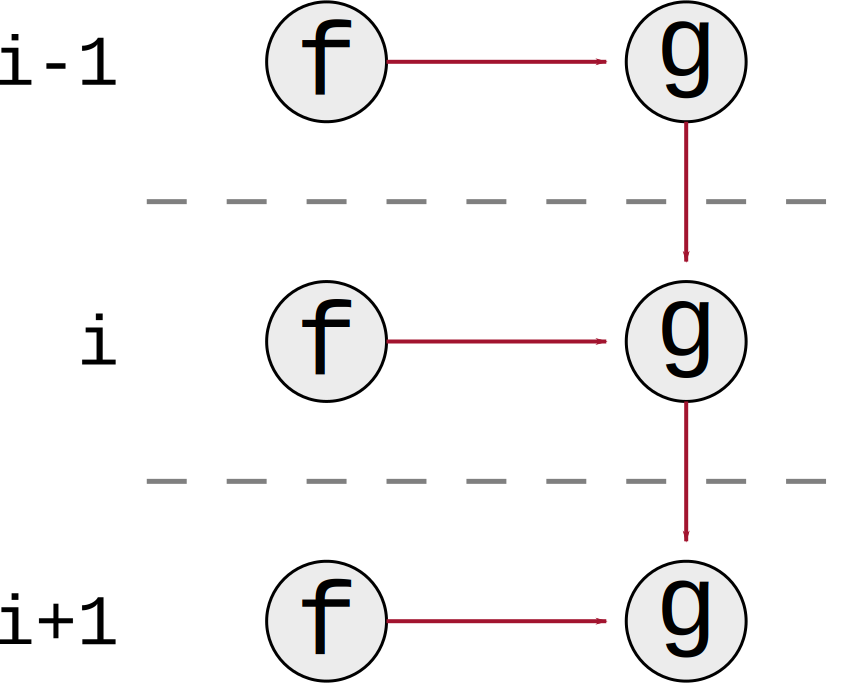
\includegraphics[width=0.8\textwidth]{figures/example_dag} \\%
        \vspace{0.8cm}
        DAG}
      %% \only<1>{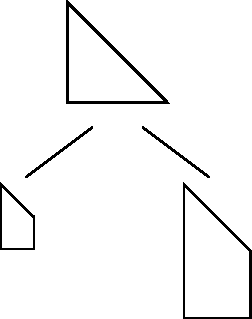
\includegraphics[width=0.6\textwidth]{figures/etree_simple}}%
      %% \only<2->{\includegraphics[width=0.6\textwidth]{figures/etree_simple_part}}%
    \end{column}
    \begin{column}{0.6\textwidth}
      \centering
      \uncover<3->{
      \includegraphics[width=0.8\textwidth]{figures/task_f} \\%
      \vspace{0.1cm}
      \includegraphics[width=0.8\textwidth]{figures/task_g} \\%
      PTG representation}
      %% \uncover<3->{\includegraphics[width=0.8\textwidth]{figures/dag}}%
    \end{column}
  \end{columns}  
\end{frame}

\begin{frame}{PTG Sparse Cholesky Factorization}
  
  \db{PTG-based} version of SpLLT implemented with \db{PaRSEC} which
  is one of the few runtime system supporting this model:

  \vspace{0.5cm}

  \begin{itemize}
    \item In PaRSEC, The PTG code is written using a dedicated
      language: \db{Job Data Flow} (JDF).

      \vspace{0.5cm}
      
    \item In a \alert{distributed-memory context}, The runtime system
      is capable of handling iter-node communications implicitly.
  \end{itemize}
    
\end{frame}

\begin{frame}{Experiments}
  \begin{center}

    \only<1>{\includegraphics[width=0.9\textwidth]{data/cmp_facto_all0}}
    \only<2->{\includegraphics[width=0.9\textwidth]{data/cmp_facto_all}}

    %% \texttt{\scriptsize
    %% \only<1>{
    %%   \begin{tabular}{r|rr|rr|rr}
    %%     \hline
    %%     \# & \multicolumn{4}{c}{spLLT}         & \multicolumn{2}{c}{MA87}                                                   \\
    %%     \hline
    %%        & \multicolumn{2}{c}{OpenMP/StarPU} & \multicolumn{2}{c}{PaRSEC} & \multicolumn{2}{c}{MA87}                      \\ 
    %%     \cline{2-7}
    %%        & nb                                & facto (s)                  & nb   & facto (s)      & nb  & facto (s)       \\
    %%     \hline
    %%     1  & 512                               & 1.801                      & 384  & 0.610          & 256 & \bf 0.376       \\
    %%     2  & 256                               & \bf 0.220                  & 384  & 0.300          & 256 & 0.252           \\
    %%     3  & 256                               & 0.205                      & 256  & 0.286          & 256 & \bf 0.194       \\
    %%     4  & 256                               & \bf 0.203                  & 384  & 0.284          & 256 & 0.213           \\
    %%     5  & 256                               & \bf 0.247                  & 256  & 0.327          & 256 & 0.259           \\
    %%     6  & 256                               & 0.267                      & 256  & 0.368          & 256 & \bf 0.257       \\
    %%     7  & 512                               & 2.631                      & 384  & 1.072          & 256 & \bf 0.586       \\
    %%     8  & 384                               & 0.812                      & 512  & 1.058          & 256 & \bf 0.786       \\
    %%     9  & 384                               & 1.186                      & 384  & 1.345          & 256 & \bf 1.111       \\
    %%     10 & 384                               & \bf 1.405                  & 512  & 1.879          & 384 & \bf 1.498       \\
    %%     11 & 384                               & \bf 2.406                  & 384  & \bf 3.673      & 512 & 3.829           \\
    %%     12 & 384                               & \bf 5.076                  & 768  & 6.333          & 384 & 5.498           \\
    %%     13 & 768                               & 7.392                      & 384  & \bf 7.061      & 384 & \bf 7.195       \\
    %%     14 & 768                               & 10.650                     & 1024 & 11.690         & 384 & \bf 10.642      \\
    %%     \hline
    %% \end{tabular}}%
    %% \only<2>{
    %%       \begin{tabular}{r|rr|rr|rr}
    %%     \hline
    %%     \# & \multicolumn{4}{c}{spLLT}         & \multicolumn{2}{c}{MA87}                                                   \\
    %%     \hline
    %%        & \multicolumn{2}{c}{OpenMP/StarPU} & \multicolumn{2}{c}{PaRSEC} & \multicolumn{2}{c}{MA87}                      \\ 
    %%     \cline{2-7}
    %%        & nb                                & facto (s)                  & nb   & facto (s)      & nb  & facto (s)       \\
    %%     \hline
    %%     1  & 512                               & 1.801                      & 384  & 0.610          & 256 & \bf 0.376       \\
    %%     2  & 256                               & \bf \dd{0.220}             & 384  & \dd{0.300}     & 256 & \dd{0.252}      \\
    %%     3  & 256                               & \dd{0.205}                 & 256  & \dd{0.286}     & 256 & \bf \dd{0.194}  \\
    %%     4  & 256                               & \bf \dd{0.203}             & 384  & \dd{0.284}     & 256 & \dd{0.213}      \\
    %%     5  & 256                               & \bf \dd{0.247}             & 256  & \dd{0.327}     & 256 & \dd{0.259}      \\
    %%     6  & 256                               & \dd{0.267}                 & 256  & \dd{0.368}     & 256 & \bf \dd{0.257}  \\
    %%     7  & 512                               & 2.631                      & 384  & 1.072          & 256 & \bf 0.586  \\
    %%     8  & 384                               & \dd{0.812}                 & 512  & \dd{1.058}     & 256 & \bf \dd{0.786}  \\
    %%     9  & 384                               & \dd{1.186}                 & 384  & \dd{1.345}     & 256 & \bf \dd{1.111}  \\
    %%     10 & 384                               & \bf \dd{1.405}             & 512  & \dd{1.879}     & 384 & \bf \dd{1.498}  \\
    %%     11 & 384                               & \bf \dd{2.406}             & 384  & \bf \dd{3.673} & 512 & \dd{3.829}      \\
    %%     12 & 384                               & \bf \dd{5.076}             & 768  & \dd{6.333}     & 384 & \dd{5.498}      \\
    %%     13 & 768                               & \dd{7.392}                 & 384  & \bf \dd{7.061} & 384 & \bf \dd{7.195}  \\
    %%     14 & 768                               & \dd{10.650}                & 1024 & \dd{11.690}     & 384 & \bf \dd{10.642} \\
    %%     \hline
    %% \end{tabular}}}
  \end{center}
  \begin{itemize}
  \item Competitive performance compared to MA87 and OpenMP/StarPU
    codes.
  \item Better performance on matrices \# 1 and \# 7 compared to
    STF-based implementations but still not as good as MA87.
  \end{itemize}
\end{frame}

\begin{frame}{Conclusion}
  \begin{itemize}
  \item The \alert{runtime-based} solver \db{SpLLT} gives competitive
    results compared to the \db{hand-tuned HSL code MA87}.

    \vspace{0.4cm}

  \item Both \alert{OpenMP} and \alert{StarPU} versions offer good
    performance but we have seen some limitations of the \db{STF
      model}.

    \vspace{0.4cm}

  \item The \alert{PTG} version also offer good performance, it
    doesn't suffer from the same limitations as the \alert{STF}-based
    codes but the code seems less efficient than the other version
    (runtime overhead ?).
  \end{itemize}
\end{frame}

\begin{frame}{Ongoing and Future work}

  \begin{itemize}
  \item Run on \alert{distributed-memory} systems: requires to provide
    a data distribution to the runtime system.

    \vspace{0.4cm}

  \item Run on \alert{GPU} and \alert{Xeon Phi} devices: requires to provide
    the computational kernels.

    \vspace{0.4cm}

  \item Handle \alert{indefinite} systems using pivoting techniques.
  \end{itemize}

\end{frame}

\begin{frame}[plain]{}
  \begin{center}
    \vspace{2cm}

    {\Huge Thanks!}

    \vspace{1cm}

    {\huge Questions?}

    \vspace{2cm}

  \end{center}
\end{frame}

\end{document}
